\documentclass[11pt, a4paper, spanish]{article}

%%%%%%%%%% COMIENZO DEL PREAMBULO %%%%%%%%%%

%Info sobre este documento
\author{Martin Cammi}
\title{Trabajo Pr'actico de Ingenier'ia del software I}

%\usepackage{infostyle}                                                  % provee un look & feel similar a un documento Word
\usepackage[top=2.5cm, bottom=2.5cm, left=2.5cm, right=2.5cm]{geometry}  % m\'argenes
\usepackage[ansinew]{inputenc}                                           % permite que los acentos del estilo \'a\'e\'i\'o\'u salgan joya
\usepackage[spanish, activeacute]{babel}                                 % idioma espa\~{n}ol, acentos f\'aciles y deletreo de palabras
\usepackage{indentfirst}                                                 % permite indentar un parrafo a mano
\usepackage{caratula}                                                    % incluye caratula est\'andar
\usepackage{graphicx}                                                    % permite insertar gr\'aficos
\usepackage{color}                                                       % permite el uso de colores en el documento
\usepackage[pdfcreator={TexLive!, LaTeX2e con TeXnicCenter y la inteligencia de Jonathan ;-)},
			pdfauthor={Grupo 2"},
			pdftitle={Base de Datos - Trabajo practico: Campeonato Sudamericano de B\'asquet},
			pdfsubject={Trabajo Practico de Modelo de Entidad Relación},
			pdfkeywords={MER, MR},
			pdfstartview=FitH,            % Fits the width of the page to the window
			bookmarksnumbered,            % los bookmarks numerados se ven mejor...
			colorlinks,                   % links con bellos colores
			linkcolor=magenta]            % permite cambiar el color de los links
			{hyperref}                    % Permite jugar con algunas cosas que aparecer\'an en el PDF final
\usepackage{hyperref}
\usepackage{rotating}
\usepackage{ulem}
\usepackage[dash]{dashundergaps}


%\selectlanguage{spanish}

\linespread{1.3}                    % interlineado equivalente al 1.5 l\'ineas de Word...
\pagestyle{myheadings}              %encabezado personalizable con \markboth{}{}
\markboth{}{Campeonato Sudamericano de B\'asquet. (Cammi, De Sousa, M\'endez, Serapio) }
\headsep = 30pt                     % separaci\'on entre encabezado y comienzo del p\'arrafo

%\addtolength{\oddsidemargin}{-2cm}	% configuracion IDEAL!!!
%\addtolength{\textwidth}{4cm}
%\addtolength{\textheight}{2cm}

% macro 'todo' para To-Do's
\def\todo#1{\textcolor{red}{#1}}

% Macro 'borde' para un texto con borde
\newsavebox{\fmbox}
\newenvironment{borde}[1]
{\begin{lrbox}{\fmbox}\begin{minipage}{#1}}
{\end{minipage}\end{lrbox}\fbox{\usebox{\fmbox}}\\[10pt]}

%%%%%%%%%% FIN DEL PREAMBULO %%%%%%%%%%

\begin{document}

\materia{Base de Datos}
\submateria{Segundo Cuatrimestre de 2012}
\titulo{Trabajo pr\'actico 1}
\subtitulo{Campeonato Sudamericano de B\'asquet.}
\grupo{Grupo 2}

\integrante{Cammi, Mart\'in}{676/02}{martincammi@gmail.com}
\integrante{De Sousa, Mariano}{389/08}{marian\_sabianaa@hotmail.com}
\integrante{M\'endez, Gonz\'alo}{843/04}{gemm83@hotmail.com}
\integrante{Serapio, Noelia}{871/03}{noeliaserapio@gmail.com}

\maketitle

\thispagestyle{empty}

\tableofcontents

\newpage

% Conviene poner las secciones como diferentes archivos,
% sobre todo cuando se trabaja en equipo.
% Es m\'as f\'acil para sincronizar mediante control de versiones.
%\input{Introducci\'on}


% BEGIN Ejemplos de uso

	%\section{Una secci\'on}
	%\label{sec:unaSeccion}
	%Hola! Soy una Secci\'on
	%	\subsection{Una subsecci\'on}
	%		Y yo soy una subsecci\'on!!!
	%		\subsubsection{Una subsubsecci\'on}
	%			Y yo soy una sub-subsecci\'on!!!
	%			\paragraph{Un p\'arrafo\\}
	%				Y yo soy un p\'arrafo, porque no hay mas sub-sub-sub-subsecciones!!!

	%\section{Otra secci\'on}
	%	Como pudimos ver en la secci\'on \ref{sec:unaSeccion}, esto es una demo de una referencia a una secci\'on.
	
	%	Tambi\'en podemos hacer referencia a la p\'agina de la secci\'on:\\[10pt]
	
		% Ejemplo de uso de un borde (falta pulir para que no tire un warning!)
	%	\begin{borde}{0.98\textwidth}
	%		En la p\'agina \pageref{sec:unaSeccion}, hay una secci\'on pilla...
	%	\end{borde}

% END Ejemplos de uso

\newpage 
\section{Tecnolog\'ia utilizada en la implementaci\'on}

    Se utiliz\'o el motor de base de datos MySql, el cual es open source y su utilizaci\'on es simple.\\

    Durante el desarrollo se observ\'o la imposibilidad que posee el motor de implementar check constraints. 
    Para poder simular esta funcionalidad se utilizaron triggers, uno previo a la inserci\'on de un nuevo registro y otro previo a la actualizaci\'on para las constraints adicionales as\'i como tambi\'en para las que se desprendieron del modelo, que tambi\'en fueron inclu\'idas en los triggers.
    Era deseable que si la check constraint fallara, el insert o update se vea cancelado, y ning\'un dato sea persistido.\\

    La forma que se encontr\'o para emular este comportamiento es llamando a un procedimiento almacenado inexistente. 
    Se produce as\'i una excepci\'on y el motor efect\'ua un rollback de los cambios efectuados en el trigger y cancela la operaci\'on de inserci\'on o actualizaci\'on.
    Tuvimos que hacer esto por la imposibilidad del motor de contar con una sentencia para mostrar un mensaje.\\

    Se agreg\'o en la base una tabla de LOG, la cual no se impacta en el modelo relacional. Pose\'ia inicialmente como objetivo la persistencia de un log sobre las inconsistencias generadas en los triggers. El inconveniente que surg\'ia es que al llamar a un procedimiento inexistente para cancelar la finalizaci\'on de un triggers, se efectuaba rollback sobre todos los cambios efectuados dentro del trigger, incluso los de la tabla de LOG (de hacerse un insert o update). Como alternativa se opt\'o por loguear las ejecuciones exitosas y visualizar por l\'inea de comandos las fallidas.
    Al tener varias condiciones a validar por trigger, estos se tornaron muy largos. La l\'ogica m\'as compleja fue extra\'ida en procedimientos almacenados. 
    Cada uno de ellos efect\'ua una llamada a uno inexistente si encuentra un error.\\

    Otro problema que encontramos fue que las claves for\'aneas no estaban habilitadas, investigando al respecto encontramos que para que funcionen las tablas deben estar creadas con el par\'ametro ENGINE en tipo InnoDB. \\

Estas fueron algunas complicaciones con las que nos encontramos al trabajar con este motor de base de datos.


\newpage 
\section{Detalles sobre el entregable}
A continuaci\'on se detalla el contenido del entregable, as\'i como su correcta utilizaci\'on.\\

\noindent{\textbf{Directorios:}}

	\begin{itemize}
		\item{\textbf{queries:}}
			\subitem{\emph{create.sql:}}
				Contiene la creaci\'on de las tablas, claves primarias y for\'aneas. 
				Se encarga autom\'aticamente de llamar a sps.sql, business\_constraints.sql, vistas.sql y data.sql (que carga los datos) en ese orden.

				\textbf{NOTA:} El nombre de la base de datos utilizada es db\_tp1. Considerar a la hora de correr este script que se borra la base de datos antes mencionada. 
				Validar antes de correrlo que no exista previamente una base con ese nombre en el servidor a correr ya que se podr\'ia perder informaci\'on.

			\subitem{\emph{sps.sql:}} Se encarga de llamar a todos los store procedures dentro del directorio sps y ejecutar su creaci\'on.

			\subitem{\emph{business\_constraints.sql:}} Se encarga de llamar a todos los archivos que generan los triggers inclu\'idos dentro del directorio llamado constraints.
				vistas.sql: ejecuta la creaci\'on de los procedimientos almacenados para el an\'alisis de los datos de manera m\'as simple y ordenada, si bien no son vistas propiamente dichas. 
				Algunas vistas disponibles:\\

				    \subitem{\textbf{partidosDeFase(idFase):}} muestra todos los partidos de esa fase.
				    \subitem{\textbf{partidosDeFaseArbitro(idFase):}} muestra todos los partidos de esa fase y los \'arbitros asignados para cada uno de ellos.\\

					Las fases v\'alidas son $1,2,3,4,5$ correspondientes a las fases\\
					FASE\_GRUPO, 5TO\_PUESTO, SEMIFINAL, 3ER\_PUESTO, FINAL respectivamente.

			\subitem{\emph{data.sql:}} Efect\'ua la carga de datos, cumpliendo con las restricciones ya inicializadas.

			\subitem{\emph{breakers.sql:}} Tiene como objeto invalidar las restricciones que se agregaron a la base. Su ejecuci\'on deberia mostrar los mensajes de error de cada constraint.

		    	\subitem{\emph{queries/contraints:} }Directorio que contiene todas las constraints implementadas a trav\'es de triggers, 
				algunos de estos archivos, ejecutan procedimientos almacenados.

		    	\subitem{\emph{queries/sps:}} Directorio que contiene todos los procedimientos almacenados para constraints subdivididos por entidad.
				Posee adem\'as dos archivos: business\_sps.sql y sp\_log\_ok.sql. El primero de ellos posee los procedimientos para la validaci\'on del \'arbitro requeridos por enunciado.
				El segundo posee el procedimiento de mantenimiento de la tabla LOG.

			    	\textbf{NOTA:} Existe un directorio adicional llamado generics que posee procedimientos de uso com\'un en varios triggers.

	\end{itemize}
\newpage 
\section{Utilizaci\'on}
\noindent{\textbf{Utilizaci\'on:}}
    A continuaci\'on se detalla la utilizaci\'on de la base para un sistema operativo Linux, 
    teniendo instalado Mysql server (para Ubuntu, el comando para descargarlo es sudo-apt get install mysql-server).\\

\begin{itemize}
    \item{Abrir una terminal.}
    \item{Posicionarse sobre el directorio queries.}
    \item{Escribir en la terminal: mysql -uroot -p[contrase\~{n}a] (contrase\~{n}a definida en la instalaci\'on del servidor).}
    \item{Ejecutar dentro del mysql server el comando source create.sql.}
\end{itemize}

Se crear\'an la base de datos, sus tablas, triggers y store procedures. Las tablas ser\'an cargadas con informaci\'on y estar\'an listas para ser consultadas.\\

\noindent{\textbf{Comandos \'utiles:}} (mysql server en Linux)

\begin{itemize}
    \item{\textbf{show databases} :} Muestra las bases de datos existentes en el servidor.
    \item{\textbf{use [db\_name]} :} Setea a db\_name como base de datos a utilizar.
    \item{\textbf{desc [table\_name]}:} Muestra el detalle de la tabla table\_name
    \item{\textbf{source [path]/file.sql}:} Corre el script inclu\'ido dentro del archivo file
    \item{\textbf{exit:}} Cierra el mysql server.
\end{itemize}

\begin{sidewaysfigure}
\section{Modelo Entidad-Relacion}
  \centering
	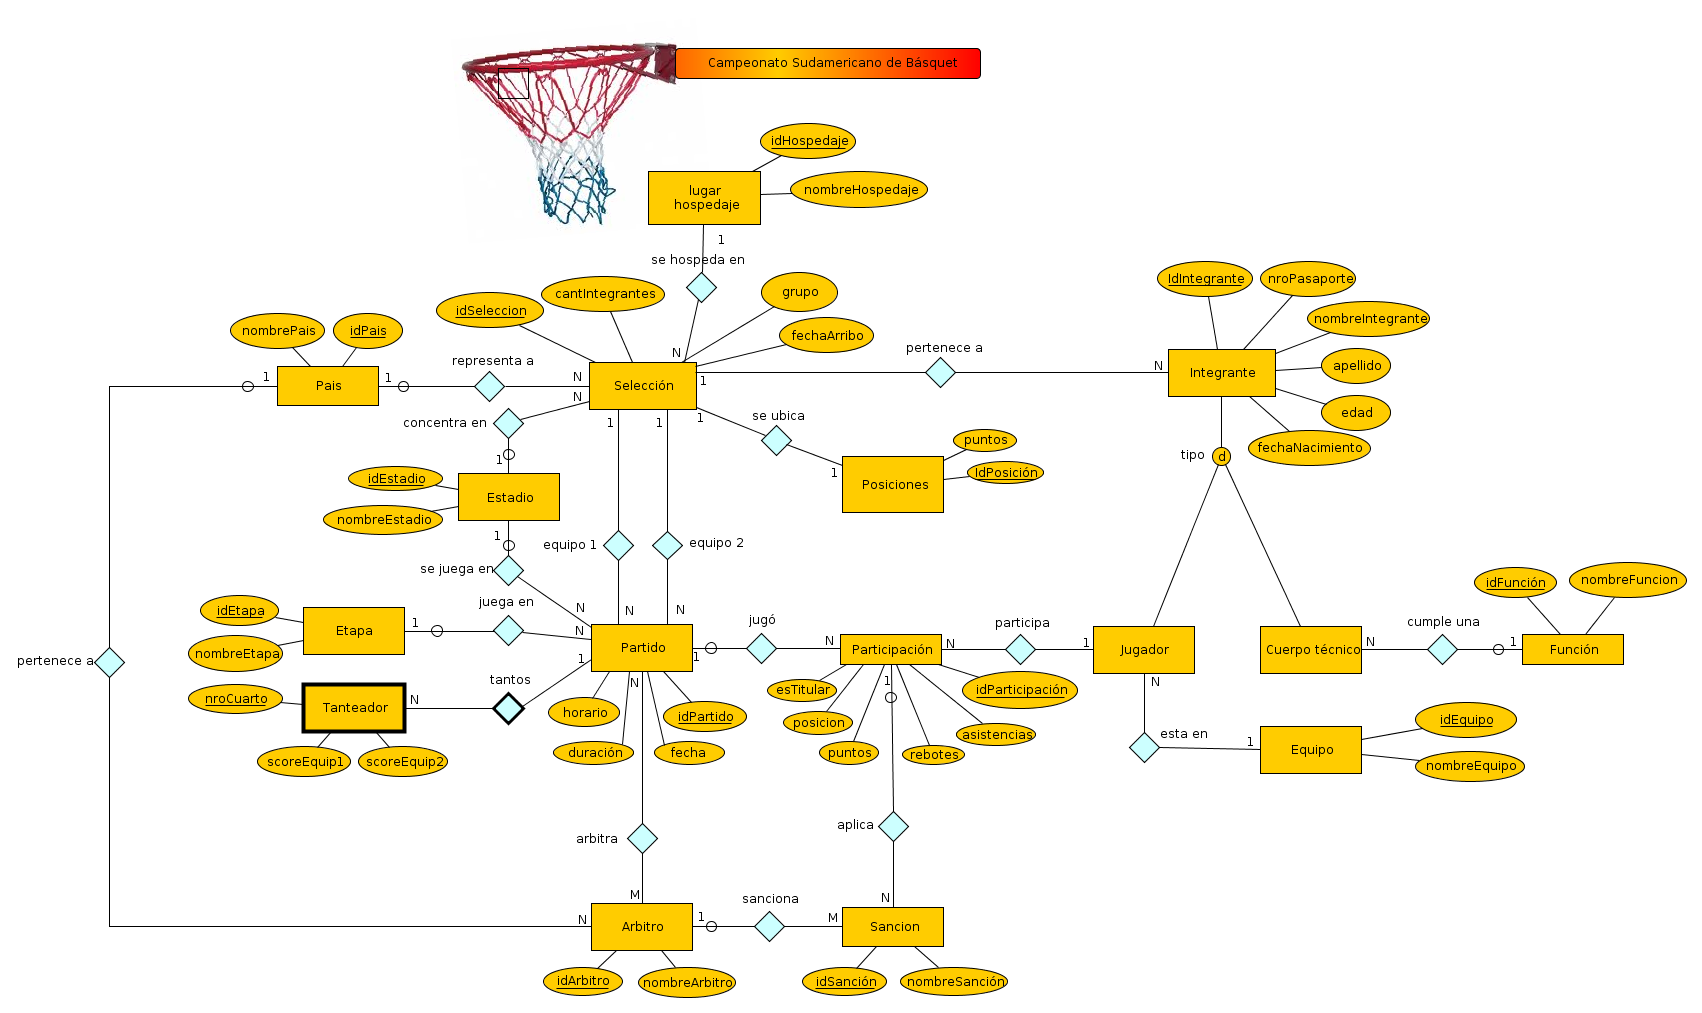
\includegraphics[scale=0.42]{diagramas/DiagramaMER.png}\\
\end{sidewaysfigure}

%	\begin{center}
%		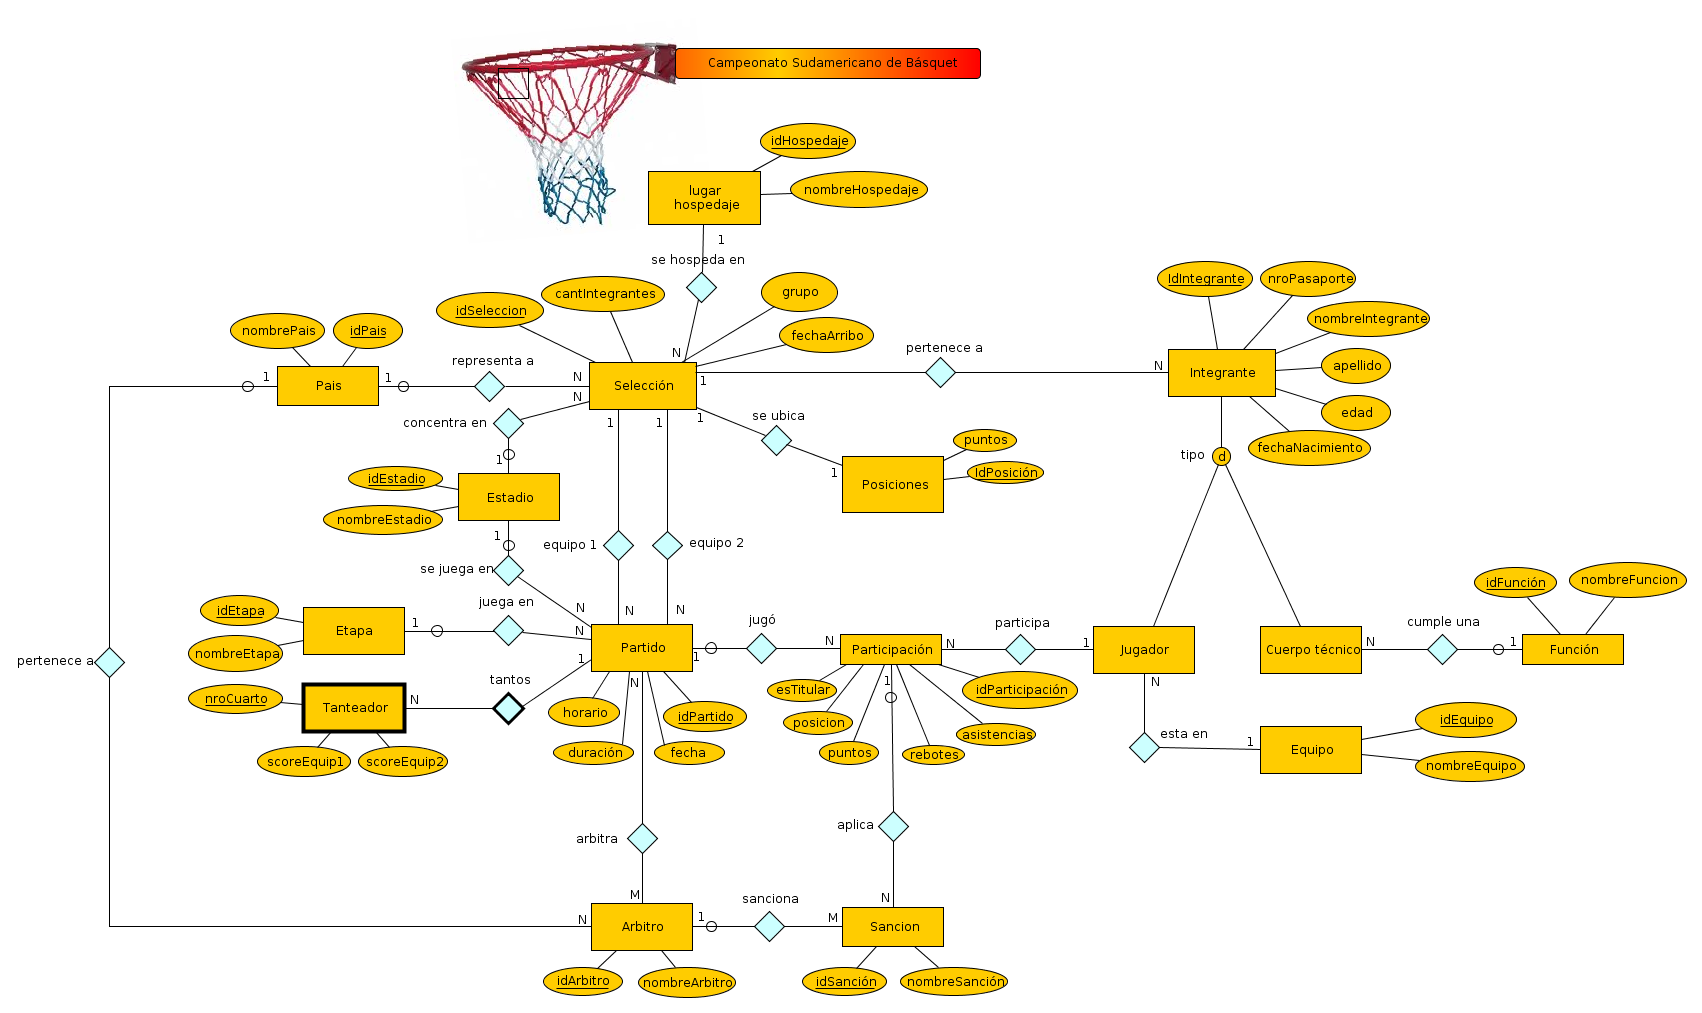
\includegraphics[scale=0.35]{diagramas/DiagramaMER.png}\\
%	\end{center}

\newpage 
\section{Modelo Logico Relacional}
\label{sec:MR}

\subsection{Entidad Selecci'on}
\textbf{SELECCION}(\underline{idSeleccion}, \dashuline{hospedaHospedaje}, \dashuline{representaPais}, \dashuline{concentraEstadio}, \dashuline{ubicaPosicion}, cantIntegrantes, fechaArribo, grupo)\\

PK = \{ (idSeleccion) \}\\
\indent{CC = \{ (idSeleccion) \}}\\
\indent{FK = \{ (hospedaHospedaje), (representaPais), (concentraEstadio), (ubicaPosicion) \}}\\

\noindent{ \textbf{References:}}

SELECCION.hospedaHospedaje debe estar en LUGARHOSPEDAJE.idHospedaje.\\ 
\indent{SELECCION.representaPais debe estar en PAIS.idPais.}\\
\indent{SELECCION.concentraEstadio debe estar en ESTADIO.idEstadio.}\\
\indent{SELECCION.ubicaPosicion debe estar en POSICION.idPosicion.}\\
\indent{SELECCION.idSeleccion debe estar en INTEGRANTE.perteneceSeleccion.} \\
\indent{SELECCION.idSeleccion debe estar en PARTIDO.equipoSeleccion1.} \\
\indent{SELECCION.idSeleccion debe estar en PARTIDO.equipoSeleccion2.} \\

\indent{SELECCION.hospedaHospedaje no puede ser nulo.}\\
\indent{SELECCION.representaPais no puede ser nulo.}\\
\indent{SELECCION.concentraEstadio no puede ser nulo.}\\
\indent{SELECCION.ubicaPosicion no puede ser nulo.}\\


\noindent{ \textbf{Constraints:}}

\indent{SELECCION.grupo $==$ ``A`` no puede repetirse m'as de 4 veces.}\\
\indent{SELECCION.grupo $==$ ``B`` no puede repetirse m'as de 4 veces.}\\
\indent{SELECCION.grupo solo puede ser ``A`` o ``B``.}\\
\indent{SELECCION.fechaArribo $<=$ PARTIDO.fecha.}\\
\indent{$\#$ SELECCION.cantIntegrantes debe ser igual a la cantidad de integrantes relacionados.}

\newpage
\subsection{Entidad Posici'on}
\textbf{POSICION}(\underline{idPosicion}, puntos, partidosJugados, partidosGanados, partidosPerdidos, tantosAFavor, tantosEnContra)\\

PK = \{ (idPosicion) \} \\
\indent{CC = \{ (idPosicion) \}} \\
\indent{FK = \{\}} \\

\noindent{ \textbf{References:}}

\indent{POSICION.idPosicion debe estar en SELECCION.ubicaPosicion.}\\

\noindent{ \textbf{Constraints:}}

\indent{POSICION.puntos $>=$ 0.}\\
\indent{POSICION.partidosJugados $>=$ 0.}\\
\indent{POSICION.partidosGanados $>=$ 0.}\\
\indent{POSICION.partidosPerdidos $>=$ 0.}\\
\indent{POSICION.partidosJugados $==$ POSICION.partidosGanados  +  POSICION.partidosPerdidos.}\\
\indent{POSICION.tantosAFavor $>=$ 0.}\\
\indent{POSICION.tantosEnContra $>=$ 0.}

\subsection{Entidad LugarHospedaje}
\textbf{LUGARHOSPEDAJE}(\underline{idHospedaje}, nombreHospedaje)\\

PK = \{ (idHospedaje) \}\\
\indent{CC = \{ (idHospedaje) \}}\\
\indent{FK = \{\}}\\

\noindent{ \textbf{References:}}

LUGARHOSPEDAJE.idHospedaje debe estar en SELECCION.hospedaHospedaje. \\

\noindent{ \textbf{Constraints:}}

\indent{Ninguna.}

\newpage
\subsection{Entidad Pa'is}
\textbf{PAIS}(\underline{idPais}, nombrePais)\\

PK = \{ (idPais) \}\\
\indent{CC = \{ (idPais) \}}\\
\indent{FK = \{\}}\\

\noindent{ \textbf{References:}}

\indent{PAIS.idPais  puede no estar en SELECCION.representaPais.}\\
\indent{PAIS.idPais  puede no estar en ARBITRO.pertenecePais.}\\

\noindent{ \textbf{Constraints:}}

\indent{Ninguna.}

\subsection{Entidad Integrante}
\textbf{INTEGRANTE}(\underline{idIntegrante}, \dashuline{perteneceSeleccion}, nroPasaporte, nombreIntegrante, apellido, fechaNacimiento,tipoIntegrante)\\

PK = \{ (idIntegrante) \} \\
\indent{CC = \{ (idIntegrante), (nroPasaporte) \}} \\
\indent{FK = \{ (perteneceSeleccion) \}} \\

\noindent{ \textbf{References:}}

\indent{INTEGRANTE.perteneceSeleccion debe estar en SELECCION.idSeleccion.} \\
\indent{INTEGRANTE.idIntegrante puede estar en JUGADOR.idJugador o (exclusivo) CUERPOTECNICO.idCuerpoTecnico.} \\

\indent{INTEGRANTE.perteneceSeleccion no puede ser nulo.} \\

\noindent{ \textbf{Constraints:}}

\indent{INTEGRANTE.tipoIntegrante IN \{ ``Jugador``, ``CuerpoTecnico`` \} .} \\
\indent{A\~{N}O(SYSDATE) $-$ A\~{N}O(INTEGRANTE.fechaNacimiento) $>=$ 18.} 

\newpage
\subsection{Entidad Jugador}
\textbf{JUGADOR}(\underline{\dashuline{idJugador}}, \dashuline{estaEnEquipo})\\

PK = \{ (idJugador) \} \\
\indent{CC = \{ (idJugador) \} }\\
\indent{FK = \{ (estaEnEquipo), (idJugador) \} }\\

\noindent{ \textbf{References:}}

\indent{JUGADOR.idJugador debe estar en INTEGRANTE.idIntegrante.} \\
\indent{JUGADOR.estaEnEquipo debe estar en  EQUIPO.idEquipo.} \\
\indent{JUGADOR.idJugador debe estar en PARTICIPACION.participaJugador.} \\


\indent{JUGADOR.estaEnEquipo no puede ser nulo.} \\

\noindent{ \textbf{Constraints:}}

\indent{Por jugador, tiene que haber una sola participaci'on en un partido.}

\subsection{Entidad CuerpoT'ecnico}
\textbf{CUERPOTECNICO}(\underline{\dashuline{idCuerpoTecnico}}, \dashuline{cumpleFuncion}) \\

PK = \{ (idCuerpoTecnico) \} \\
\indent{CC = \{ (idCuerpoTecnico) \} } \\
\indent{FK = \{ (cumpleFuncion), (idCuerpoTecnico) \} } \\

\noindent{ \textbf{References:}}

\indent{CUERPOTECNICO.idCuerpoTecnico debe estar en INTEGRANTE.idIntegrante.} \\
\indent{CUERPOTECNICO.cumpleFuncion debe estar en FUNCION.idFuncion.} \\

\indent{CUERPOTECNICO.cumpleFuncion no puede ser nulo.} \\

\noindent{ \textbf{Constraints:}}

\indent{Ninguna.}

\newpage
\subsection{Entidad Funci'on}
\textbf{FUNCION}(\underline{idFuncion}, nombreFuncion) \\

PK = \{ (idFuncion) \} \\
\indent{CC = \{ (idFuncion) \} }  \\
\indent{FK = \{\} } \\

\noindent{ \textbf{References:}}

\indent{FUNCION.idFuncion puede no estar en CUERPOTECNICO.cumpleFuncion. \\

\noindent{ \textbf{Constraints:}}

\indent{Ninguna.}

\subsection{Entidad Equipo}
\textbf{EQUIPO}(\underline{idEquipo}, nombreEquipo) \\

PK = \{ (idEquipo) \} \\
\indent{CC = \{ (idEquipo) \} }\\
\indent{FK = \{\} }\\

\noindent{ \textbf{References:}}

\indent{EQUIPO.idEquipo debe estar en JUGADOR.estaEnEquipo.} \\

\noindent{ \textbf{Constraints:}}

\indent{Ninguna}

\newpage
\subsection{Entidad Partido}
\textbf{PARTIDO}(\underline{idPartido}, \dashuline{juegaEnEtapa}, \dashuline{equipoSeleccion1}, \dashuline{equipoSeleccion2}, \dashuline{juegaEnEstadio}, duracion, fecha, horario) \\

PK = \{ (idPartido) \} \\
\indent{CC = \{ (idPartido) \} \\
\indent{FK = \{ (juegaEnEtapa), (equipoSeleccion1), (equipoSeleccion2), (juegaEnEstadio) \} \\

\noindent{ \textbf{References:}}

\indent{PARTIDO.juegaEnEtapa debe estar en ETAPA.idEtapa.} \\
\indent{PARTIDO.equipoSeleccion1 debe estar en SELECCION.idSeleccion.} \\
\indent{PARTIDO.equipoSeleccion2 debe estar en SELECCION.idSeleccion.} \\
\indent{PARTIDO.juegaEnEstadio debe estar en ESTADIO.idEstadio.} \\
\indent{PARTIDO.idPartido debe estar en ARBITRA.idPartidoArb.} \\ 
\indent{PARTIDO.idPartido puede no estar en PARTICIPACION.jugoPartido.} \\
\indent{PARTIDO.idPartido debe estar en TANTEADOR.idPartido.} \\

\indent{PARTIDO.juegaEnEtapa no puede ser nulo.} \\
\indent{PARTIDO.equipoSeleccion1 no puede ser nulo.} \\
\indent{PARTIDO.equipoSeleccion2 no puede ser nulo.} \\
\indent{PARTIDO.juegaEnEstado no puede ser nulo.} \\

\noindent{ \textbf{Constraints:}}

\indent{PARTIDO.equipoSeleccion1 $<>$ PARTIDO.equipoSeleccion2.} \\
\indent{Si PARTIDO.juegaEnEtapa $==$ ``FASE\_GRUPOS`` $\Rightarrow$  PARTIDO.equipoSeleccion1.grupo $==$ PARTIDO.equipoSeleccion2.grupo.} \\
\indent{Si PARTIDO.juegaEnEtapa $==$ ``FASE\_GRUPOS`` $\Rightarrow$  $\#$ PARTIDO $<=$ 12.} \\
\indent{Si PARTIDO.juegaEnEtapa $==$ ``5TO\_PUESTO`` $\Rightarrow$  $\#$ PARTIDO $<$= 1.} \\
\indent{Si PARTIDO.juegaEnEtapa $==$ ``3ER\_PUESTO`` $\Rightarrow$  $\#$ PARTIDO $<=$ 1.} \\
\indent{Si PARTIDO.juegaEnEtapa $==$ ``SEMIFINAL`` $\Rightarrow$  $\#$ PARTIDO $<=$ 2.} \\
\indent{Si PARTIDO.juegaEnEtapa $==$ ``FINAL`` $\Rightarrow$  $\#$ PARTIDO $<=$ 1.} \\
\indent{No puede haber dos partidos en un mismo horario.} \\
\indent{Validar que al insertar un partido, esten todos los anteriores de fase.} \\
\indent{Las fechas de los partidos tienen que estar ordenado por la etapa (FASE\_GRUPO $<$ 5TO\_PUESTO $<$ SEMIFINAL $<$ 3ER\_PUESTO $<$ FINAL).} \\
\indent{La duraci'on de los partidos tiene que ser $>$ 0.} \\
\indent{La hora del partido tiene que estar entre 0 y 23.} \\
\indent{Dos equipos no pueden enfrentarse en la misma etapa dos veces.} \\

\subsection{Entidad Estadio}
\textbf{ESTADIO}(\underline{idEstadio}, nombreEstadio) \\

PK = \{ (idEstadio) \} \\
\indent{CC = \{ (idEstadio) \} }\\
\indent{FK = \{\} } \\

\noindent{ \textbf{References:}}

ESTADIO.idEstadio puede no estar en PARTIDO.juegaEnEstadio. \\
ESTADIO.idEstadio puede no estar en SELECCION.concentraEstadio. \\

\noindent{ \textbf{Constraints:}}

\indent{Ninguna.}

\subsection{Entidad Etapa}

\textbf{ETAPA}(\underline{idEtapa}, nombreEtapa)

PK = \{ (idEtapa) \} \\
\indent{CC = \{ (idEtapa) (nombreEtapa) \} } \\
\indent{FK = \{\} } \\

\noindent{ \textbf{References:}}

ETAPA.idEtapa puede no estar en PARTIDO.juegaEnEtapa. \\

\noindent{ \textbf{Constraints:}}

ETAPA.nombreEtapa debe ser o bien FASE\_GRUPOS o 5TO\_PUESTO, o 3ER\_PUESTO o SEMIFINAL, o FINAL. 

\newpage
\subsection{Entidad Tanteador}
\textbf{TANTEADOR}(\underline{nroCuarto}, \underline{\dashuline{idPartido}}, scoreEquip1, scoreEquip2)

PK = \{ (nroCuatro, idPartido) \} \\
\indent{CC = \{ (nroCuarto,idPartido) \} } \\
\indent{FK = \{ (idPartido) \} } \\

\noindent{ \textbf{References:}}

TANTEADOR.idPartido debe estar en PARTIDO.idPartido. \\

\indent{TANTEADOR.idPartido no puede ser nulo. \\

\noindent{ \textbf{Constraints:}}

Los valores posibles de TANTEADOR.nroCuatro son \{1 ,2 , 3, 4\}. \\ 
\indent{TANTEADOR.scoreEquip1 $>=$ 0.} \\  
\indent{TANTEADOR.scoreEquip2 $>=$ 0.} \\ 
\indent{Si TANTEADOR.nroCuarto $==$ 4 $\Rightarrow$ TANTEADOR.scoreEquip1 $<>$ TANTEADOR.scoreEquip2 (no hay empates).} \\   

\noindent{ \textbf{Constraints Adicionales:}}

\indent{TANTEADOR.nroCuarto no puede aparecer m'as de 4 veces por  TANTEADOR.idPartido (el tanteador se genera con los 4 cuartos cuando se genera un partido). }  

\newpage
\subsection{Entidad Arbitro}
\textbf{ARBITRO}(\underline{idArbitro}, \dashuline{pertenecePais}, nombreArbitro)

PK = \{ (idArbitro) \} \\
\indent{CC = \{ (idArbitro) \} } \\
\indent{FK = { (pertenecePais) \} } \\

\noindent{ \textbf{References:}}

\indent{ARBITRO.pertenecePais debe estar en PAIS.idPais.} \\
\indent{ARBITRO.idArbitro debe estar en ARBITRA.idArbitroArb.} \\ 
\indent{ARBITRO.idArbitro puede no estar en SANCION.sancionadaPorArbitro.} \\ 

\indent{ARBITRO.pertenecePais no puede ser nulo.} \\

\noindent{ \textbf{Constraints:}}

\indent{Ninguna.} \\

\noindent{ \textbf{Constraints Adicionales:}} 

Un 'arbitro no puede dirigir un partido si: 
\begin{itemize}
\item Dirigi'o a alguno de los equipos 2 o m'as veces, y en todos los partidos el equipo obtuvo el mismo resultado (gan'o o perdi'o, no hay empate).
\item Dirigi'o una sola vez a cada equipo con resultados opuestos.        
\item Est'a asignado a dirigir un partido en la misma fecha.    
\end{itemize}

\subsection{Entidad Arbitra}
\textbf{ARBITRA}(\underline{\dashuline{idArbitroArb}}, \underline{\dashuline{idPartidoArb}})

PK = \{ (idArbitroArb, idPartidoArb) \} \\
\indent{CC = \{ (idArbitroArb, idPartidoArb) \} } \\
\indent{FK = \{ (idArbitroArb), (idPartidoArb) \} } \\

\noindent{ \textbf{References:}}

ARBITRA.idArbitroArb debe estar en ARBITRO.idArbitro. } \\
\indent{ARBITRA.idPartidoArb debe estar en PARTIDO.idPartido. } \\

\noindent{ \textbf{Constraints:}}

(ARBITRO.idArbitro $==$ ARBITRA.idArbitroArb) and (ARBITRA.idPartidoArb $==$ PARTIDO.idPartido) $\Rightarrow$  (ARBITRO.pertenecePais $<>$ PARTIDO.seleccionEquipo1.representaPais and ARBITRO.pertenecePais $<>$ PARTIDO.seleccionEquipo2.representaPais). 

\newpage
\subsection{Entidad Participaci'on}
\textbf{PARTICIPACION}(\underline{idParticipacion}, \dashuline{jugoPartido}, \dashuline{participaJugador}, asistencias, rebotes, posicion, puntos, esTitular)

PK = \{ (idParticipacion) \} \\
\indent{CC = \{ (idParticipacion) \} } \\
\indent{FK = \{ (jugoPartido), (participaJugador) \} } \\

\noindent{ \textbf{References:}}

PARTICIPACION.jugoPartido debe estar en PARTIDO.idPartido. \\
\indent{PARTICIPACION.participaJugador debe estar en JUGADOR.idJugador.} \\
\indent{PARTICIPACION.idParticipacion puede no estar en SANCION.aplicaParticipacion.} \\
\indent{PARTICIPACION.posicion puede ser o bien BASE o ESCOLTA o ALERO o ALA-PIVOT o PIVOT o nulo.} \\

\indent{PARTICIPACION.jugoPartido no puede ser nulo.} \\
\indent{PARTICIPACION.participaJugador no puede ser nulo.} \\

\noindent{ \textbf{Constraints:}}

PARTICIPACION.jugoPartido.equipoSeleccion1 puede aparecer a lo sumo 5 veces con PARTICIPACION.esTitular $==$ true. \\
(Esta resticci\'on no fue modelada en la implementaci\'on f\'isica)\\

\indent{PARTICIPACION.jugoPartido.equipoSeleccion2 puede aparecer a lo sumo 5 veces con PARTICIPACION.esTitular $==$ true.} \\
(Esta resticci\'on no fue modelada en la implementaci\'on f\'isica)\\

\indent{No puede haber dos PARTICIPACION.participaJugador tal que PARTICIPACION.esTitular $==$ true y  PARTICIPACION.participaJugador.IdIntegrante.perteneceSeleccion  sean iguales y PARTICIPACION.posicion sean iguales.} \\
\indent{PARTICIPACION.rebotes $>=$ 0.} \\
(Esta resticci\'on no fue modelada en la implementaci\'on f\'isica)\\

\indent{PARTICIPACION.asistencias $>=$ 0.} \\ 
\indent{PARTICIPACION.puntos $>=$ 0.}  \\
\indent{Si PARTICIPACION.esTitular $==$ false $\Rightarrow$ PARTICIPACION.posicion is null.} 
(Esta resticci\'on no fue modelada en la implementaci\'on f\'isica)\\

\subsection{Entidad Sanci'on}
\textbf{SANCION}(\underline{idSancion}, \dashuline{aplicaParticipacion}, \dashuline{sancionadaPorArbitro}, \dashuline{esDeTipo})

PK = \{ (idSancion) \} \\
\indent{CC = \{ (idSancion) \} } \\
\indent{FK = \{ (aplicaParticipacion) , (sancionadaPorArbitro), (esDeTipo) \} } \\

\noindent{ \textbf{References:}}

SANCION.aplicaParticipacion debe estar en PARTICIPACION.idParticipacion.} \\
\indent{SANCION.sancionadaPorArbitro debe estar en ARBITRO.idArbitro.} \\
\indent{SANCION.esDeTipo debe estar en TIPOSANCION.idTipoSancion.} \\

\indent{SANCION.aplicaParticipacion no puede ser nulo.} \\
\indent{SANCION.sancionadaPorArbitro no puede ser nulo.} \\
\indent{SANCION.esDeTipo no puede ser nulo.} \\

\noindent{ \textbf{Constraints:}}

\indent{ARBITRA.idArbitroArb $==$ SANCION.sancionadaPorArbitro  and ARBITRA.idPartidoArb $==$  SANCION.aplicaParticipacion.jugoPartido.} 

\subsection{Entidad TipoSanci'on}
\textbf{TIPOSANCION}(\underline{idTipoSancion}, nombreSancion)\\

PK = \{ (idTipoSancion) \} \\
\indent{CC = \{ (idTipoSancion) \} } \\
\indent{FK = \{\} } \\

\noindent{ \textbf{References:}}

\indent{TIPOSANCION.idTipoSancion puede no estar en SANCION.esDeTipo.} \\

\noindent{ \textbf{Constraints:}}

\indent{Ninguna.}

\newpage 
\section{Esquema de partidos}
    A continuaci\'on se detalla cu\'ales son los partidos, selecciones y resultados obtenidos utilizando la carga de datos suministrada en el informe (data.sql).\\

\begin{figure}[hb]
	\begin{center}
		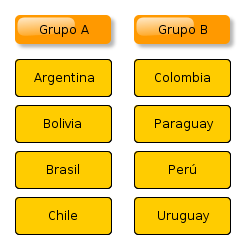
\includegraphics[scale=0.6]{diagramas/grupos.png}\\
		\caption{Grupos del torneo}
	\end{center}

	\begin{center}
		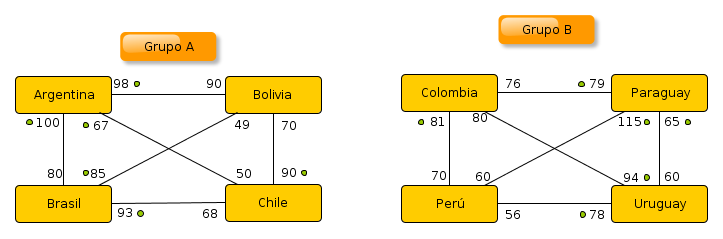
\includegraphics[scale=0.6]{diagramas/partidoDeFase.png}\\
		\caption{Partidos de Fase de grupos}
	\end{center}
$\qquad$
$\qquad$
$\qquad$
$\qquad$
	\begin{center}
		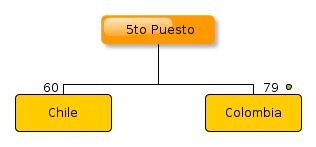
\includegraphics[scale=0.6]{diagramas/partido5toPuesto.png}\\
		\caption{Partido de 5to puesto}
	\end{center}
\end{figure}

\begin{figure}
	\centering
	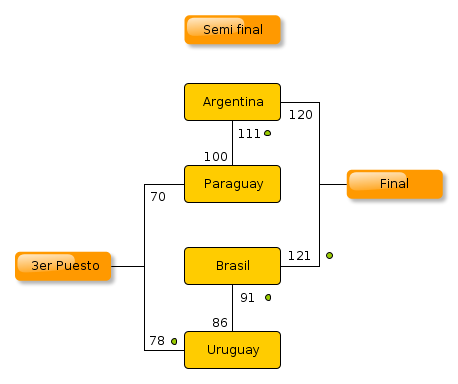
\includegraphics[scale=0.6]{diagramas/partidoSemi3erYFinal.png}\\
	\caption{Partido de 5to puesto}
\end{figure}

\newpage 
\section{Decisiones tomadas y supuestos asumidos}

	Se agreg\'o la entidad Posici\'on, entidad que posee todos sus atributos redundates (estos pueden ser inferidos del modelo relacional sin la entidad Posici\'on, de manera no trivial). \\
	Se decidi\'o agregarla ya que la informaci\'on suministrada define el resultado final del Torneo de Basquet.\\

La informaci\'on que suministra, depende de la cantidad de partidos jugados, la etapa de cada uno de ellos y qui\'en fue el ganador.\\

Teniendo esta entidad redundante en el modelo, las consultas sobre el resultado final del Torneo se simplifican considerablemente, y no deben ser recalculadas para cada una de ellas.

    Para el c\'alculo de la tabla de posiciones se defini\'o arbitrariamente los siguientes puntajes por partidos ganados:\\

\indent{Partido ganado en \textbf{FASE\_GRUPO} $\Rightarrow$ 1 punto.}\\
\indent{Partido ganado en \textbf{5TO\_PUESTO} $\Rightarrow$ 3 puntos.}\\
\indent{Partido ganado en \textbf{SEMIFINAL} $\Rightarrow$ 7 puntos.}\\
\indent{Partido ganado en \textbf{3ER\_PUESTO} $\Rightarrow$ 11 puntos.}\\
\indent{Partido ganado en \textbf{FINAL} $\Rightarrow$ 19 puntos.}\\

    Internamente se insertan 4 las filas en el tanteador por cada vez que se inserta un partido.\\

    El c\'alculo de la tabla de posiciones se hace internamente al hacer update de los valores del \'ultimo cuarto en el tanteador al terminar un partido. 
    De esta manera y para preservar consistencia, una vez insertado estos resultados, ellos no pueden ser editados. Cuando el \'ultimo partido (la final) haya sido jugado y terminado, la entidad posici\'on contar\'a con toda la informaci\'on sobre el campeonato.\\

    Se modela la entidad \textbf{TipoSancion} para agrupar los tipos de sanciones ya que consideramos que probable que en un futuro pueda agregarse una sanci\'on nueva.
    Los hospedajes salvados, corresponden a los indicados por los jugadores.\\

    S\'olo se guardan los equipos correspondientes a los jugadores de la selecciones.


\newpage 
\section{Dise\~{n}o f\'isico}

A continuaci\'on se detalla mediante un gr\'afico cu\'al fue el dise\~{n}o de base de datos elegido para representar el modelo relacional.

 
\begin{figure}[hb]
  \centering
  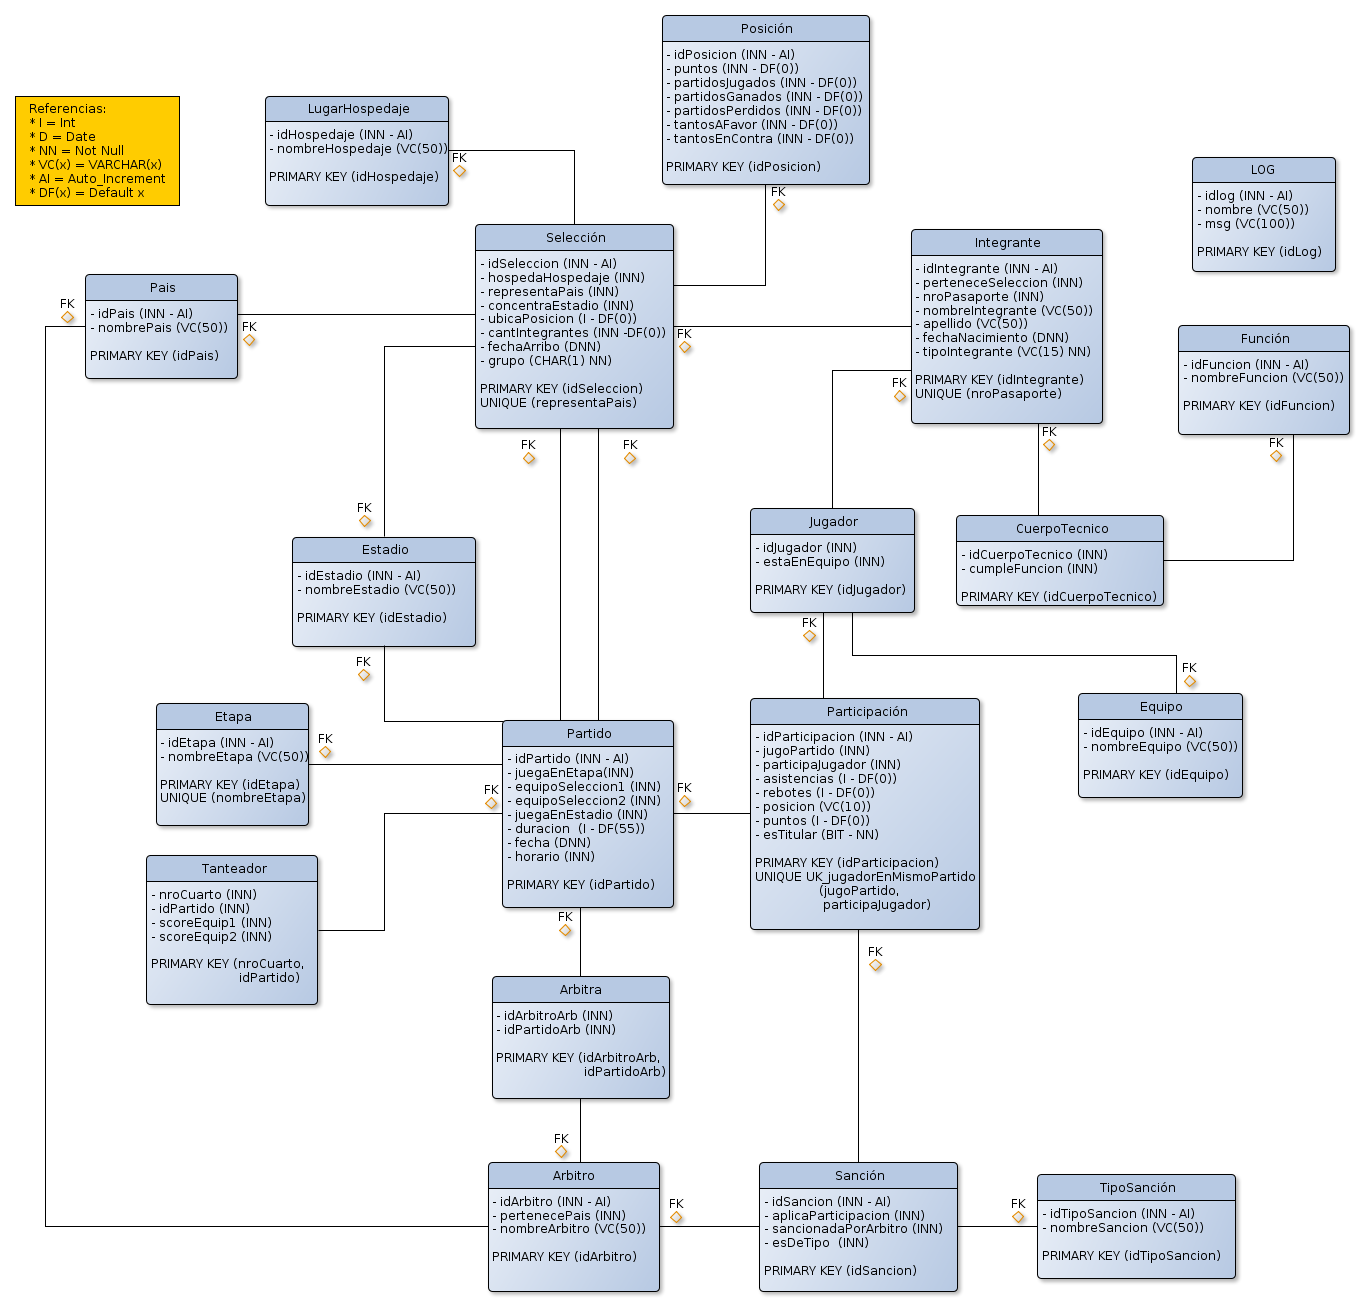
\includegraphics[scale=0.37]{diagramas/DiagramaFisico.png}\\
\end{figure}

%	\begin{center}
%		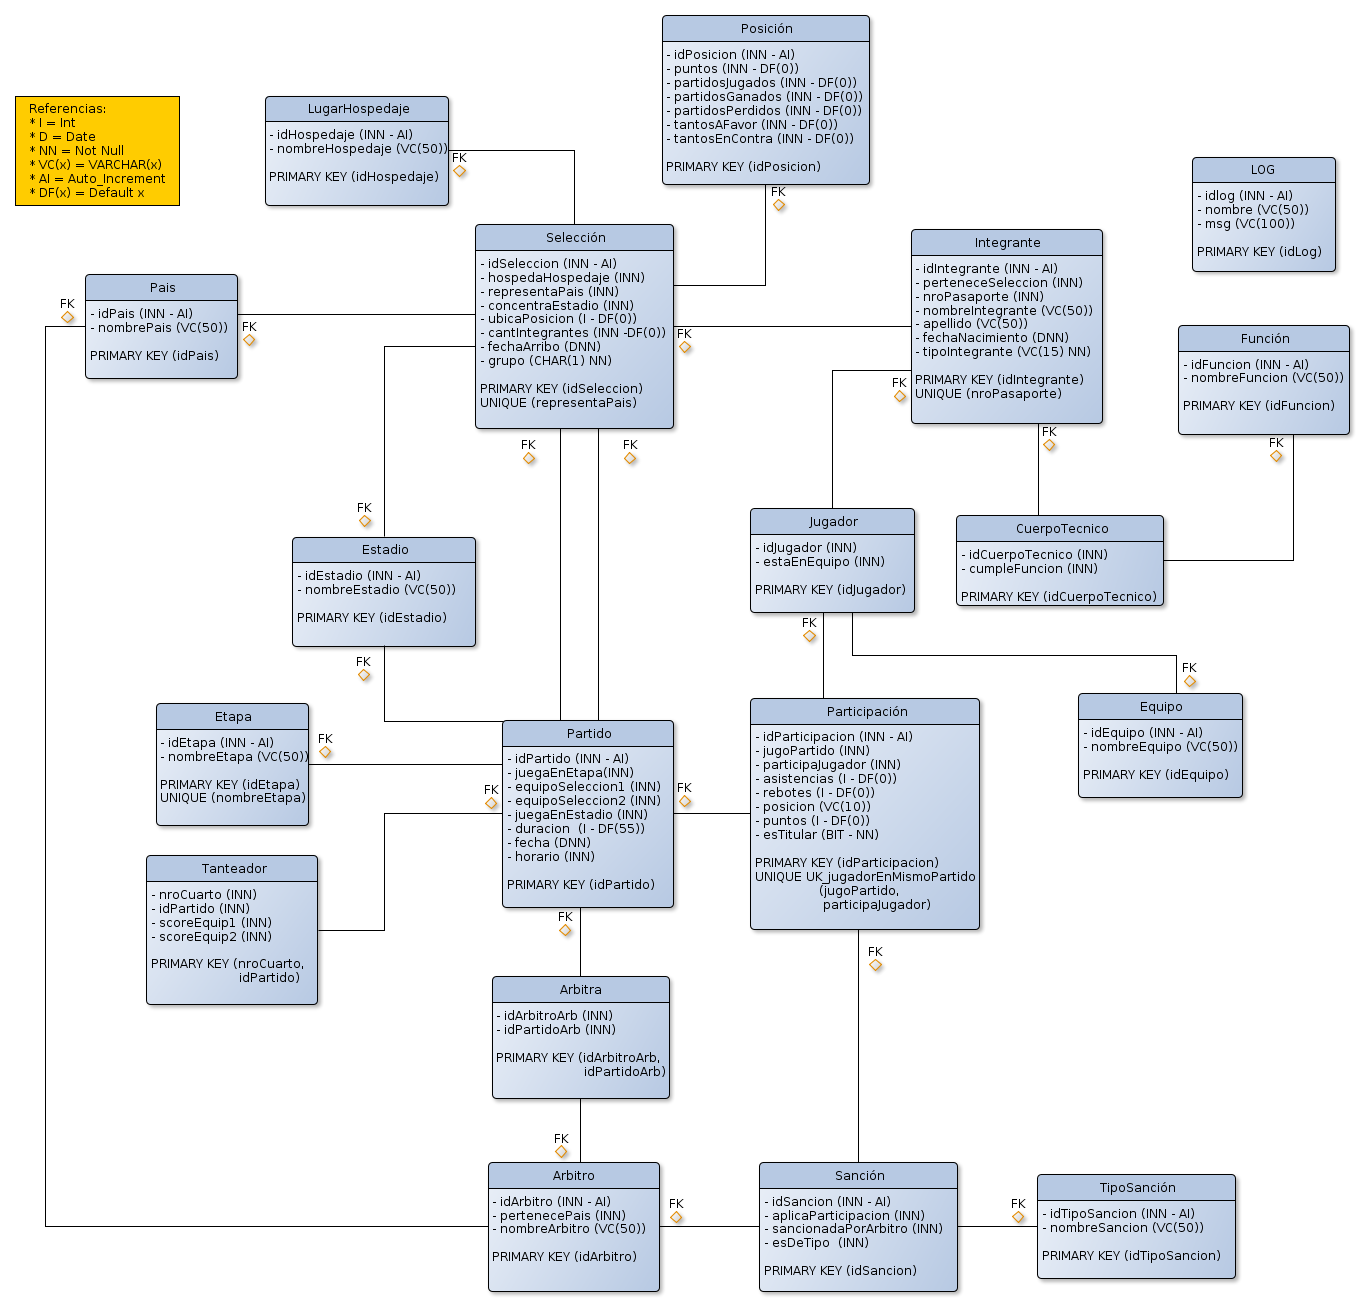
\includegraphics[scale=0.45]{diagramas/DiagramaFisico.png}\\
%	\end{center}



\newpage 
\section{Breakers}

Los breakers son sentencias de inserts dise\~{n}adas espec\'ificamente para poner a prueba las restricciones del modelo.
El archivo breakers.sql permite ejecutarlas y ver como todas ellas se verifican.

\section{Restricciones al modelo}

\subsection{Restricciones pedidas por la c\'atedra}

\begin{itemize}
	\item{Una consulta que devuelva todos los nombres de los pa\'ises cuyos equipos utilizaron a todos sus jugadores en alg\'un partido como titulares.\\
	    	Esta restricci\'on se encuentra modelada en el archivo \textbf{business\_sps.sql} y el store procedure se llama \textbf{sp\_paises\_todos\_titulares()}
	}

	\item{Un reporte con los nombres de los jugadores, la cantidad de partidos en que particip\'o y los promedios de puntos, asistencias y rebotes. 
		El reporte debe estar ordenado por  cantidad de partidos en que participo cada jugador.\\
		Esta restricci\'on se encuentra modelada en el archivo \textbf{business\_sps.sql} y el store procedure se llama \textbf{sp\_estadisticas\_por\_jugador()}
	}

	\item{A medida que va avanzando un torneo, se van cargando en la BD los pr\'oximos
		partidos, y asignando \'arbitros a los mismos. Un \'arbitro no puede dirigir un partido si:
		\begin{itemize}
			\item{Dirigi\'o a alguno de los equipos 2 o m\'as veces, y en todos los partidos el equipo obtuvo el mismo resultado (gan\'o o perdi\'o, no hay empate)}
			\item{Dirigi\'o una sola vez a cada equipo con resultados opuestos.}
			\item{Est\'a asignado a dirigir un partido en la misma fecha}
		\end{itemize}
		Se pide realizar un stored procedure que dado un partido, devuelva los \'arbitros candidatos a dirigirlo. \\
		Esta restricci\'on se encuentra modelada en el archivo \textbf{business\_sps.sql} y el store procedure se llama \textbf{sp\_posibles\_arbitros\_por\_partidos(idPartidoSP INT)}
	}

	\item{Implementar una restricci\'on que impida que en la base de datos se pueda asignar un \'arbitro en un partido que sea del mismo pa\'is
	     	que alguno de los equipos que participa. \\
	     	Esta restricci\'on se encuentra modelada en el archivo \textbf{arbitraConstraints.sql} y el trigger se llama \textbf{check\_arbitra\_bi}
	}

	\item{Implementaci\'on de alguna restricci\'on adicional que surja del dise\~{n}o. 
		En el archivo \textbf{business\_constraints.sql} se encuentran detalladas todas las constraints adicionales que se han creado.
	}

\end{itemize}

\newpage
\subsection{Restricciones adicionales al modelo}

	Contamos con m\'as de 40 restricciones al modelo de entre las cuales se encuentran las dictadas por el Modelo de entidad relaci\'on y por restricciones propias agregadas
	descriptas en la secci\'on de Modelo l\'ogico relacional~\ref{sec:MR}


\end{document}
